\documentclass[../main.tex]{subfiles}
\begin{document}
在一个欧几里得空间中,任一针对点空间的点的等距变换结果都是相对某另一点的平移再叠加一个正交变换。这个定理也是后面介绍物理定律的标架变换不变性时的理论基础。我们把它正式表述如下:

\begin{theorem}[等距变换的表示定理]\label{thm:II.3.2}
    设$\mathcal{E}$是一个欧几里得空间,$\mathcal{V}$是其平移空间,$\mathcal{I}$就$\mathcal{E}$的等距群。选定任一点$X_0\in\mathcal{E}$,$\mathcal{E}$上的任一等距变换$i:\mathcal{E}\rightarrow\mathcal{E},i\in\mathcal{I}$都可表示为
    \[
        i\left(X\right)=i\left(X_0\right)+\mathbf{Q}_i\left(X-X_0\right)
    \]
    其中$\mathbf{Q}_i$是一个正交算符,由$i$唯一确定。
\end{theorem}
\begin{proof}
    见附录。
\end{proof}

由定理\ref{thm:II.3.2},给定欧几里得空间上的任一等距变换$i$,仅需知道$i$关于某一参考点$X_0$的像是哪个点$i\left(X_0\right)$,以及由$i$确定的某特征正交算符$\mathbf{Q}_i$的取值,就可以知道$i$对任意一点$X\in\mathcal{E}$的像$i\left(X\right)$。享有表示定理的等距变换$i$未必需要是$\mathcal{V}$中的向量,但由于任意两点的“差”唯一对应一个$\mathcal{V}$中的平移向量,故$i\left(X\right)-i\left(X_0\right)$和$X-X_0$分别表示由点$i\left(X_0\right)$到点$i\left(X\right)$和点$X_0$到点$X$的平移向量。由等距变换的表示定理,这两个平移向量只相差由正交算符$\mathbf{Q}_i$规定的几何变换,具体是什么几何变换,可回顾\S\ref{sec:II.3.3}。

\begin{figure}[ht]
    \centering
    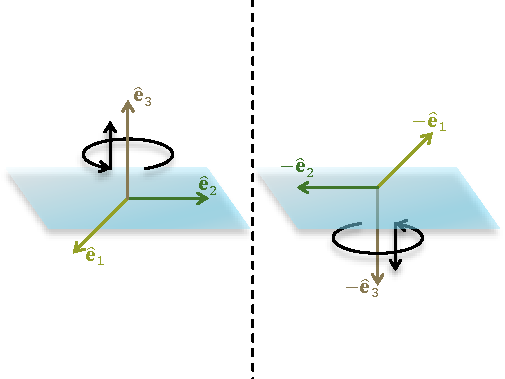
\includegraphics[width=0.5\textwidth]{images/II.3.3.pdf}
    \caption{翻转变换在纸面画法上相当于左、右手规则之差别。}
    \label{fig:II.3.4}
\end{figure}

\begin{example}\label{exp:II.3.4}
    考虑欧几里得空间$\left(\mathcal{E},d\right)$上的以下等距变换,其中$\mathbf{Q}$是一个正交算符,$X_0,C$是$\mathcal{E}$中固定的点:
    \begin{align*}
        i_1\left(X\right) & =X+\left(C-X_0\right)                \\
        i_2\left(X\right) & =X_0+\mathbf{Q}\left(X-X_0\right)    \\
        i_3\left(X\right) & =X+\mathbf{Q}^{-1}\left(C-X_0\right)
    \end{align*}

    $i_1$把任一点向固定的方向平移固定距离($i_1\left(X\right)=X+\mathbf{u},\mathbf{u}\equiv C-X_0$)。

    $i_1\circ i_2=i_2\circ i_3$(自行验证作为练习。)

    当$\mathbf{Q}=\mathbf{I}$时,$i_2$是恒等映射。当$\mathbf{Q}\neq\mathbf{I}$时,由正交算符性质$\mathrm{det}\mathbf{Q}=\pm 1$。当$\mathrm{det}\mathbf{Q}=1$时,$i_2$是一种旋转操作;当$\mathrm{det}\mathbf{Q}=-1$时,由$\mathbf{Q}=\left(-\mathbf{I}\right)\left(-\mathbf{Q}\right)$和$\mathrm{det}\left(-\mathbf{Q}\right)=1$可知$i_2$是先进行了一个旋转($-\mathbf{Q}$)再进行了反转($-\mathbf{I}$)的操作。
\end{example}

由该例最后的结论可知,$\mathrm{det}\mathbf{Q}$为$+1$和$-1$的两种情况,只差一个翻转$-\mathbf{I}$变换。设$\left\{\mathbf{\hat{e}}_1,\mathbf{\hat{e}}_2,\mathbf{\hat{e}}_3\right\}$是3维欧几里得空间的平移空间$\mathcal{V}$的一组规范正交基,则它们经过翻转变换后形成的另一组基$\left\{-\mathbf{\hat{e}}_1,-\mathbf{\hat{e}}_2,-\mathbf{\hat{e}}_3\right\}$,在画法惯例上只存在“左手规则”与“右手规则”的差别(图\ref{fig:II.3.4})。用形象的语言说,就是我们的物理世界是存在“镜子外”和“镜子内”两套的,而且它们的运动学规律只相差一个翻转变换。在本讲义内,我们只关心“镜子外的物理世界”的规律,并规定用“右手规则”来建立坐标系,对应于$\mathrm{det}\mathbf{Q}=1$的情况。基于同样的惯例,“叉乘”运算$\mathbf{a}\times\mathbf{b}$得到的向量方向也是按“右手规则”得到。
\end{document}